\documentclass[12pt,a4paper]{article}

\usepackage[T1,T2A]{fontenc}
\usepackage[utf8]{inputenc}
\usepackage[english, russian]{babel}
\usepackage{indentfirst}
\usepackage{misccorr}
\usepackage{graphicx}
\usepackage{amsmath}
\usepackage{graphicx}
\usepackage{float}
\usepackage[left=20mm,right=10mm, top=20mm,bottom=20mm,bindingoffset=0mm]{geometry}

\setlength{\parskip}{6pt}\graphicspath{{images/}}\DeclareGraphicsExtensions{.png}

\begin{document}

    \begin{titlepage}
        \begin{center}
            \large
            Санкт-Петербургский политехнический университет\\Петра Великого\\
            \vspace{0.5cm}
            Физико-механический институт\\
            \vspace{0.25cm}
            Кафедра «Прикладная математика»
            \vfill
            \textsc{\LARGE\textbf{Отчет по лабораторной работе №4}}\\[5mm]
            \Large
            по дисциплине\\"Математическая статистика"
        \end{center}
        \vfill
        \begin{tabular}{l p{175pt} l}
            Выполнил студент \\ группы 5030102/00101 && Нгуен Хоанг Линь
            \vspace{0.25cm}
            \\Проверил \\ доцент, к.ф.-м.н. && Баженов Александр Николаевич
        \end{tabular}
        \vfill
        \begin{center}
            Санкт-Петербург \\ 2023 г.
        \end{center}
    \end{titlepage}
    
\newpage
\begin{center}
    \tableofcontents
    \setcounter{page}{2}
\end{center}
\newpage
\begin{center}
    \listoffigures
\end{center}

\newpage
\section{Постановка задачи}
Для 5 распределений:
\begin{itemize}
    \item Нормальное распределение $N(x,0,1)$
    \item Распределение Коши $C(x,0,1)$
    \item Распределение Лапласа $L(x,0,\frac{1}{\sqrt{2}})$
    \item Распределение Пуассона $P(k,10)$
    \item Равномерное распределение $U(x,-\sqrt{3},\sqrt{3})$
\end{itemize}

Необходимо:
\begin{enumerate}
    \item Сгенерировать выборки размером 20, 60 и 100 элементов
    \item Построить на них эмпирические функции распределения и ядерные оценки плотности распределения на отрезке $[-4, 4]$ для непрерывных распределений и на отрезке $[6, 14]$ для распределения Пуассона
\end{enumerate}

\section{Теория}
\subsection{Эмпирическая функция распределения}
\textit{Статистический ряд} - последовательность различных элементов выборки ${\{z_i\}}_{i=1}^k$, расположенных по возрастанию, с указанием частот ${\{n_i\}}_{i=1}^k$, с которыми эти элементы содержатся в выборке. Обычно записывается в виде таблицы.

\textit{Эмпирическая (выборочная) функция распределения} - относительная частота события $X<x$, полученная по данной выборке:
\begin{equation}
    F_n^*(x)=P^*(X<x)
\end{equation}

Для получения относительной частоты $P^*(X < x)$ просуммируем в статистическом ряде, построенном по данной выборке, все частоты $n_i$, для которых элементы $z_i$ статистического ряда меньше $x$. Тогда $P^*(X < x) = \frac{1}{n}\sum_{z_i<x}n_i$. Получаем:
\begin{equation}
    F^*(x)=\frac{1}{n}\sum_{z_i<x}n_i
\end{equation}
где $F^*(x)-$ функция распределения дискретной случайной величины $X^*$, заданной таблицей распределения:
\begin{table}[H]
    \centering
    \begin{tabular}{|c|c|c|c|c|}
        \hline
         $X^*$ & $z_1$ & $z_2$ & ... & $z_k$\\
         \hline
         $P$ & $\frac{n_1}{n}$ & $\frac{n_2}{n}$ & ... & $\frac{n_k}{n}$\\
         \hline
    \end{tabular}
    \caption{Таблица распределения}
\end{table}
Эмпирическая функция распределения является оценкой, т. е. приближённым значением, генеральной функции распределения
\begin{equation}
F_n^*(x)\approx F_X(x)
\end{equation}

\subsection{Ядерные оценки плотности вероятности}
\textit{Оценкой плотности вероятности $f(x)$} называется функция $\widehat{f}(x)$, построенная на основе выборки, приближенно равная $f(x)$
\begin{equation}
\widehat{f}(x)\approx f(x)
\end{equation}

Представим оценку в виде суммы с числом слагаемых, равным объёму выборки:
\begin{equation}
    \widehat{f}_n(x)=\frac{1}{n h_n}\sum_{i=1}^n{K(\frac{x-x_i}{h_n})}
\end{equation}
Здесь функция $K(u)$ - ядро (ядерная функция), непрерывна и является плотностью вероятности, $x_1,...,x_n$ - элементы выборки, любая последовательность положительных чисел $\{h_n\}$, обладающая свойствами:
\begin{equation}
    h_n\xrightarrow[n\to\infty]{}0;
    n h_n\xrightarrow[n\to\infty]{}\infty.
\end{equation}
Такие оценки называются непрерывными ядерными

Гауссово (нормальное) ядро:
\begin{equation}
    K(u)=\frac{1}{\sqrt{2\pi}}e^{-\frac{u^2}{2}}
\end{equation}

Правило Сильвермана:
\begin{equation}
    h_n=1.06\hat{\sigma}n^{-1/5}
\end{equation}
где $\hat{\sigma}$ - выборочное стандартное отклонение.

\section{Реализация}
Лабораторная работа выполнена на языке Python в виртуальной среде Anaconda с интерпретатором версии 3.9 в среде разработки Visual Studio Code. Дополнительные зависимости:
\begin{itemize}
    \item scipy
    \item numpy
    \item matplotlib
    \item seaborn
    \item statsmodels
\end{itemize}


\section {Результаты}
\subsection{Эмпирическая функция распределения}
\begin{figure}[H]
    \centering
    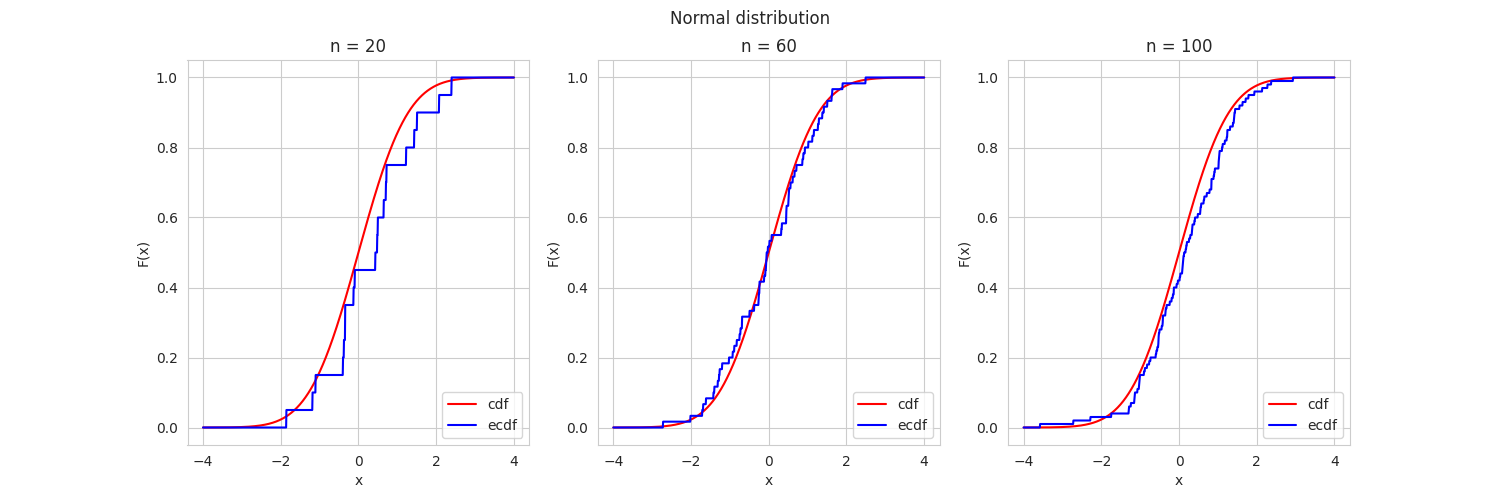
\includegraphics[scale=0.5]{Normal_cdf.png}
    \caption{Нормальное распределение}
\end{figure}

\begin{figure}[H]
    \centering
    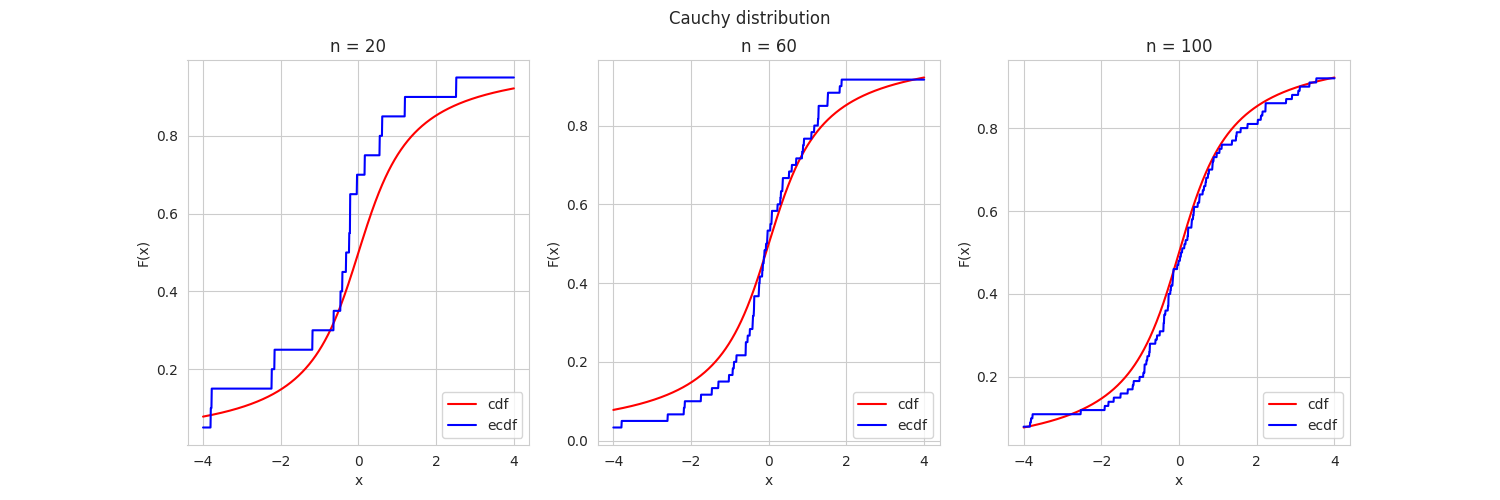
\includegraphics[scale=0.5]{Cauchy_cdf.png}
    \caption{Распределение Коши}
\end{figure}

\begin{figure}[H]
    \centering
    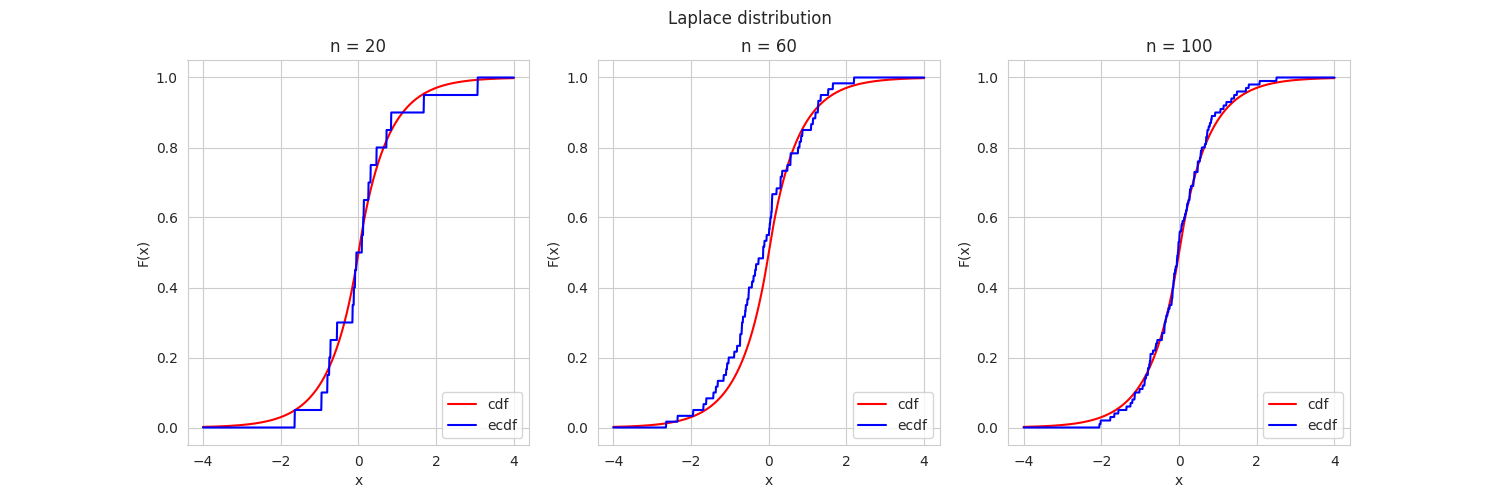
\includegraphics[scale=0.5]{Laplace_cdf.png}
    \caption{Распределение Лапласа}
\end{figure}

\begin{figure}[H]
    \centering
    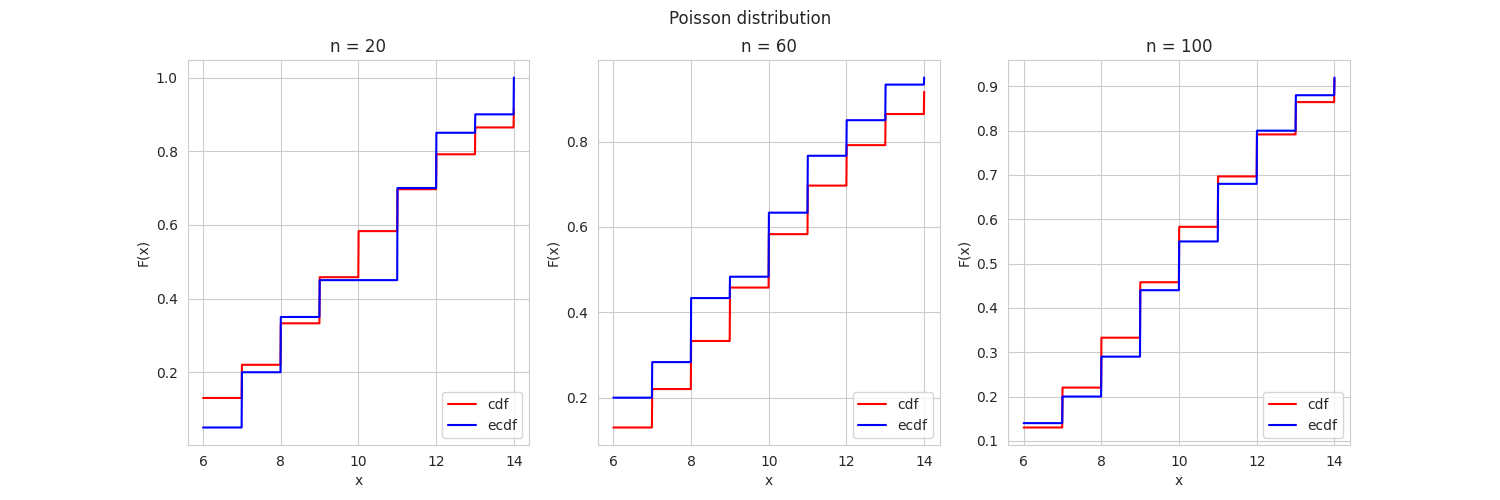
\includegraphics[scale=0.5]{Poisson_cdf.png}
    \caption{Распределение Пуассона}
\end{figure}

\begin{figure}[H]
    \centering
    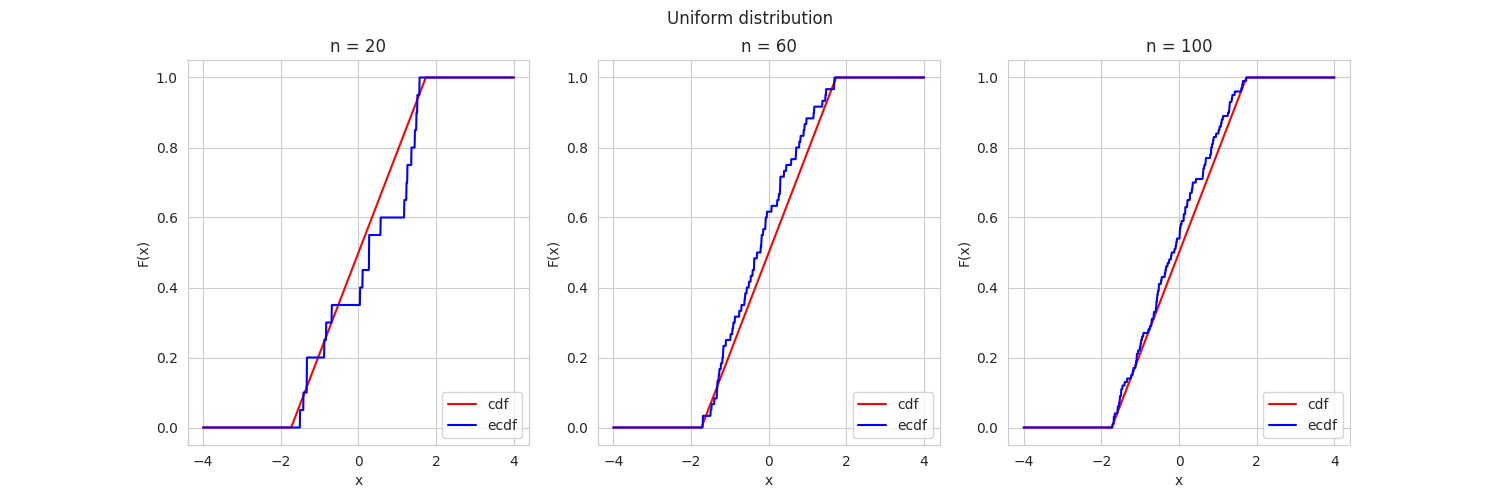
\includegraphics[scale=0.5]{Uniform_cdf.png}
    \caption{Равномерное распределение}
\end{figure}

\subsection{Ядерные оценки плотностей распределения}
\begin{figure}[H]
    \centering
    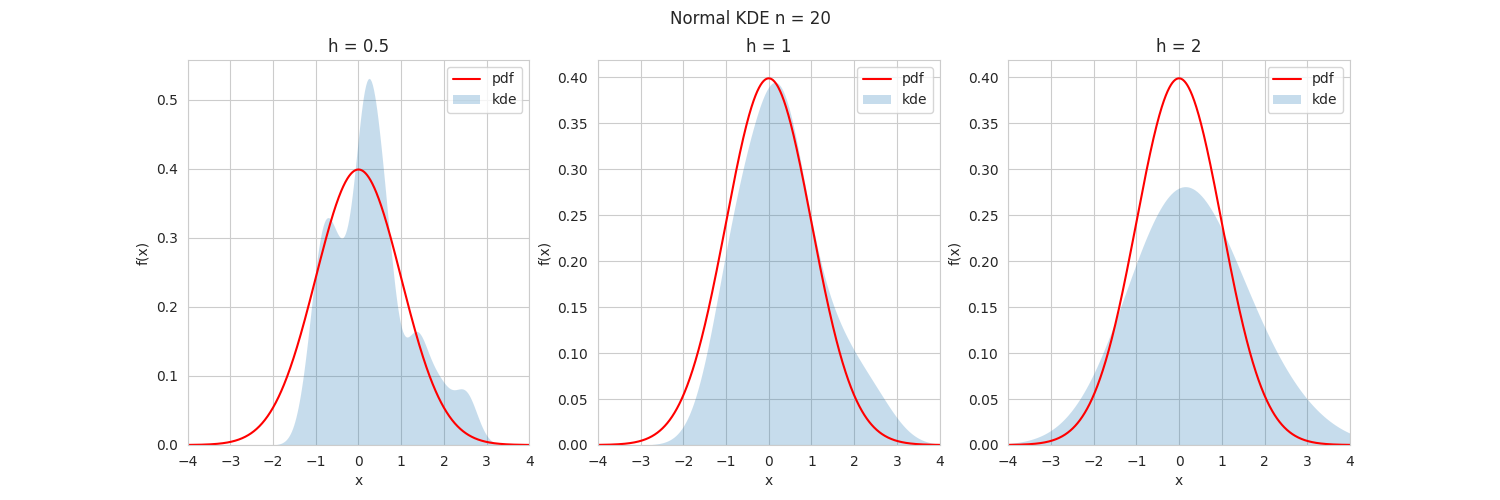
\includegraphics[scale=0.5]{Normal_pdf_20.png}
    \caption{Нормальное распределение размерностью 20}
\end{figure}

\begin{figure}[H]
    \centering
    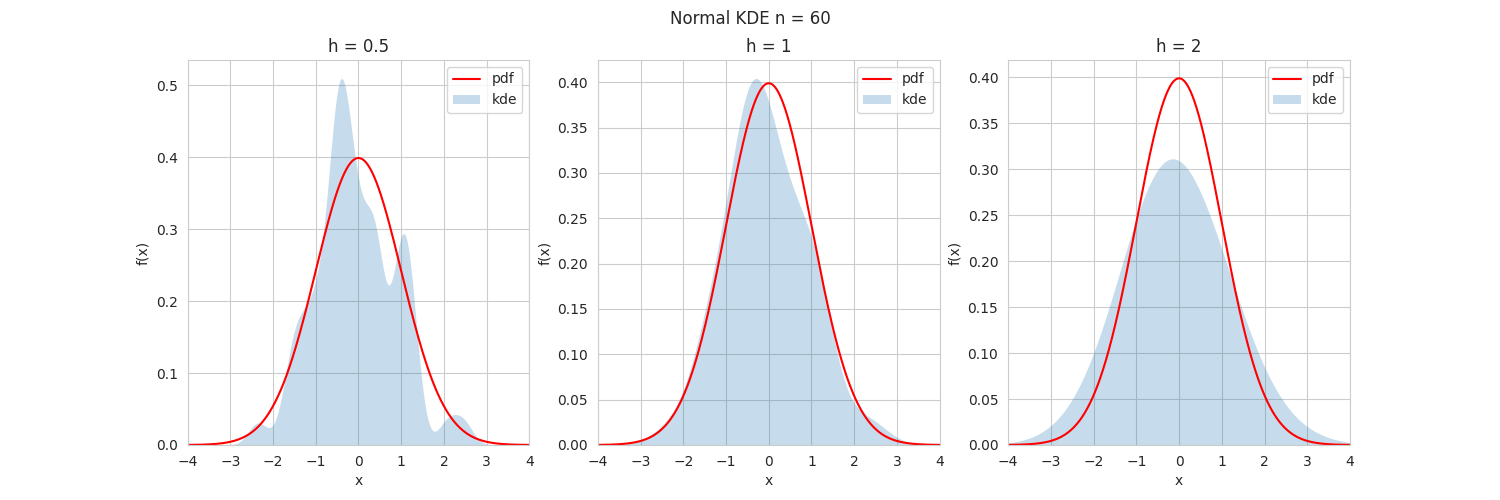
\includegraphics[scale=0.5]{Normal_pdf_60.png}
    \caption{Нормальное распределение размерностью 60}
\end{figure}

\begin{figure}[H]
    \centering
    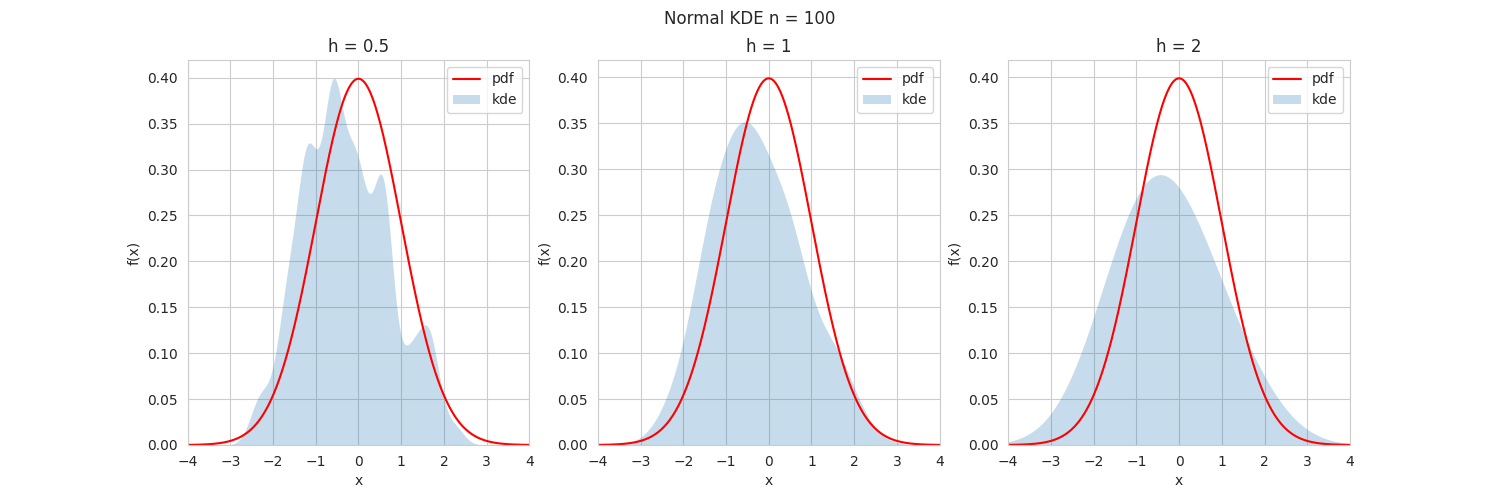
\includegraphics[scale=0.5]{Normal_pdf_100.png}
    \caption{Нормальное распределение размерностью 100}
\end{figure}

\begin{figure}[H]
    \centering
    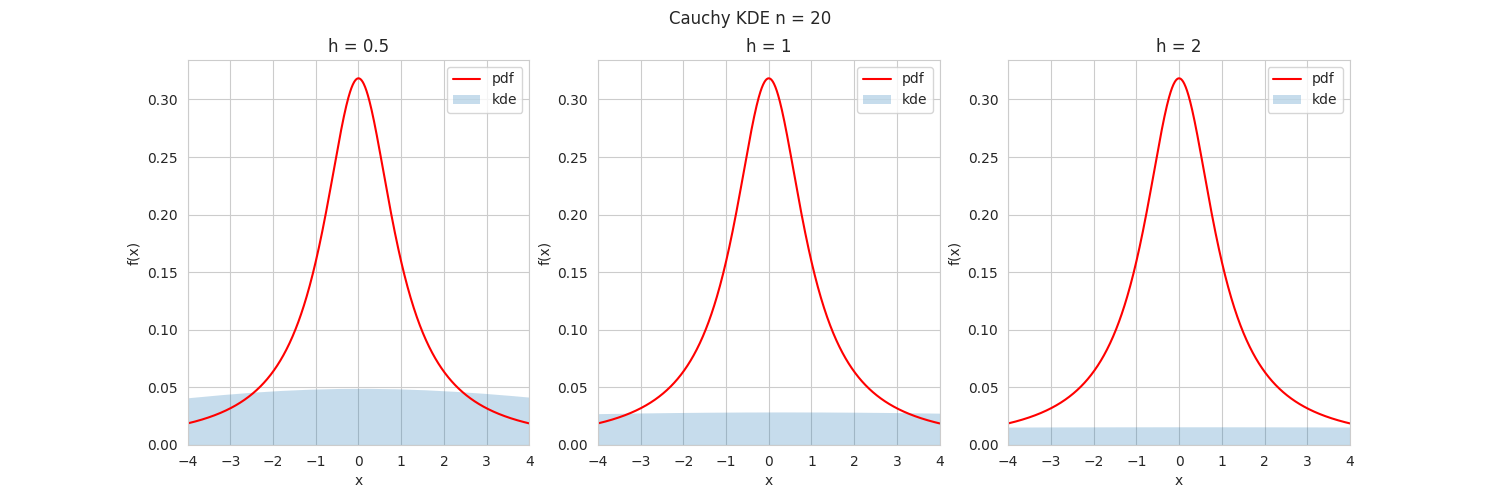
\includegraphics[scale=0.5]{Cauchy_pdf_20.png}
    \caption{Распределение Коши размерностью 20}
\end{figure}

\begin{figure}[H]
    \centering
    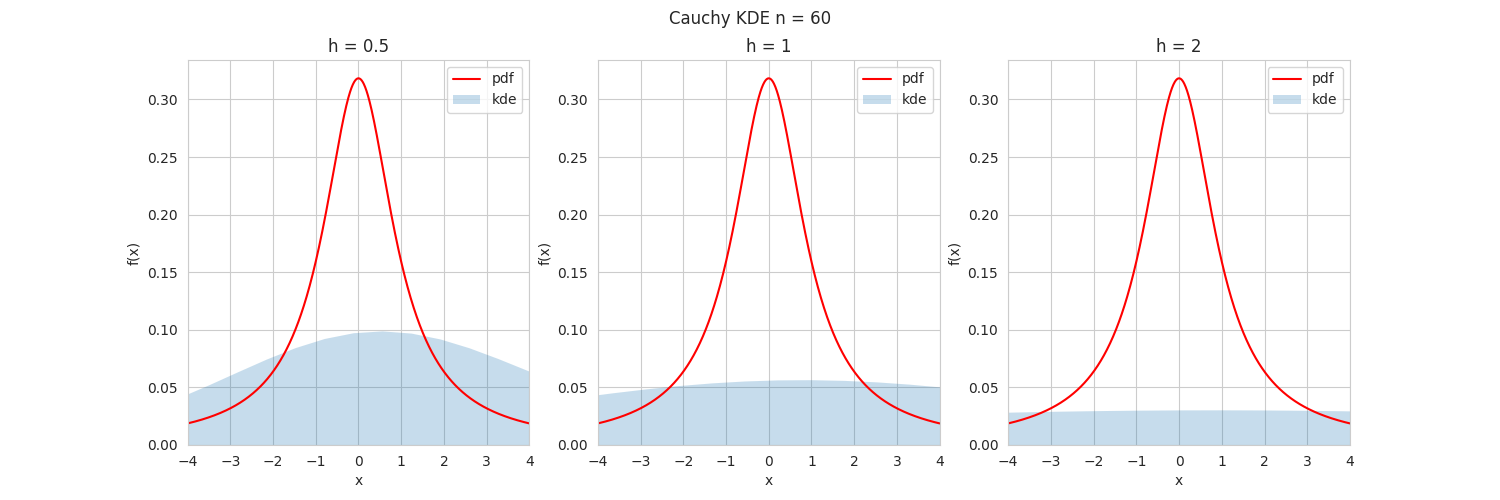
\includegraphics[scale=0.5]{Cauchy_pdf_60.png}
    \caption{Распределение Коши размерностью 60}
\end{figure}

\begin{figure}[H]
    \centering
    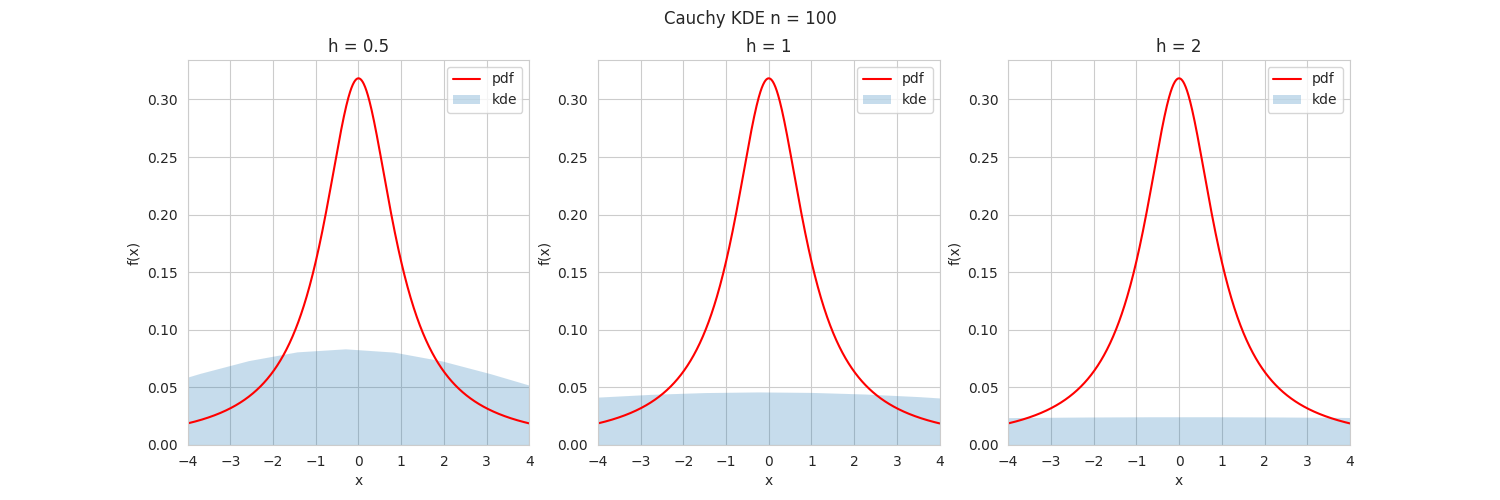
\includegraphics[scale=0.5]{Cauchy_pdf_100.png}
    \caption{Распределение Коши размерностью 100}
\end{figure}

\begin{figure}[H]
    \centering
    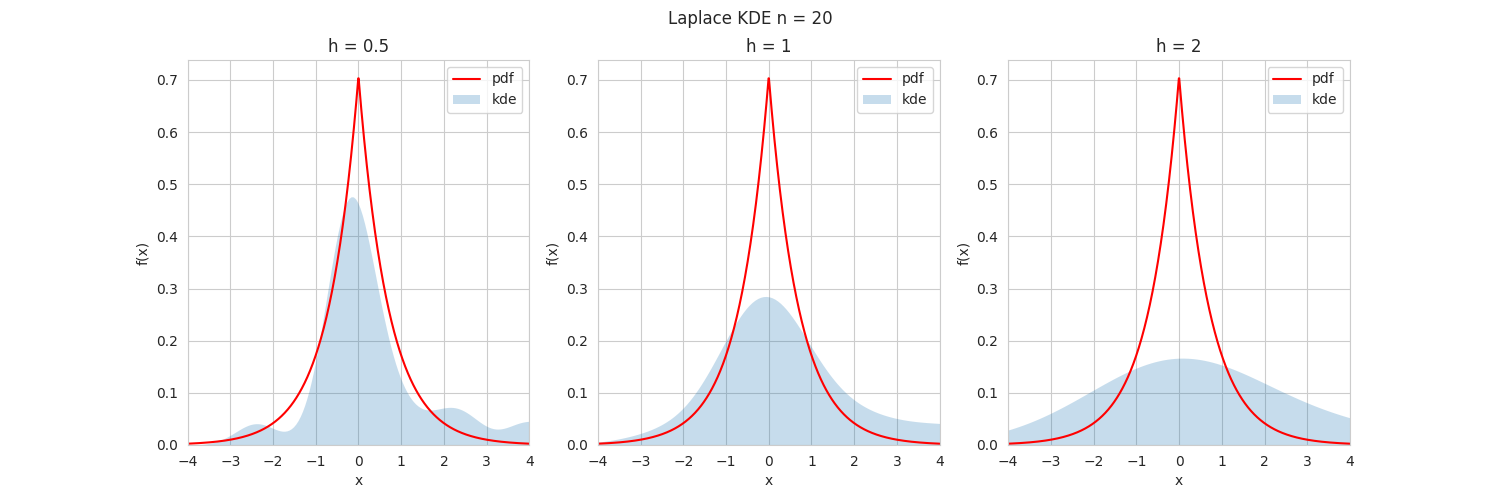
\includegraphics[scale=0.5]{Laplace_pdf_20.png}
    \caption{Распределение Лапласа размерностью 20}
\end{figure}

\begin{figure}[H]
    \centering
    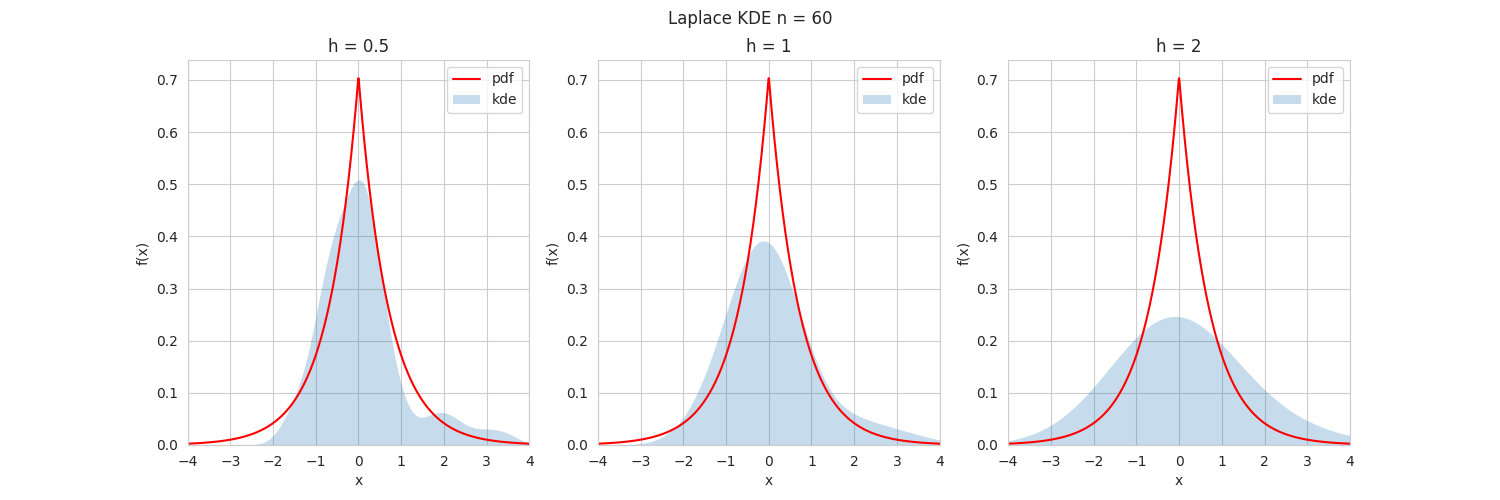
\includegraphics[scale=0.5]{Laplace_pdf_60.png}
    \caption{Распределение Лапласа размерностью 60}
\end{figure}

\begin{figure}[H]
    \centering
    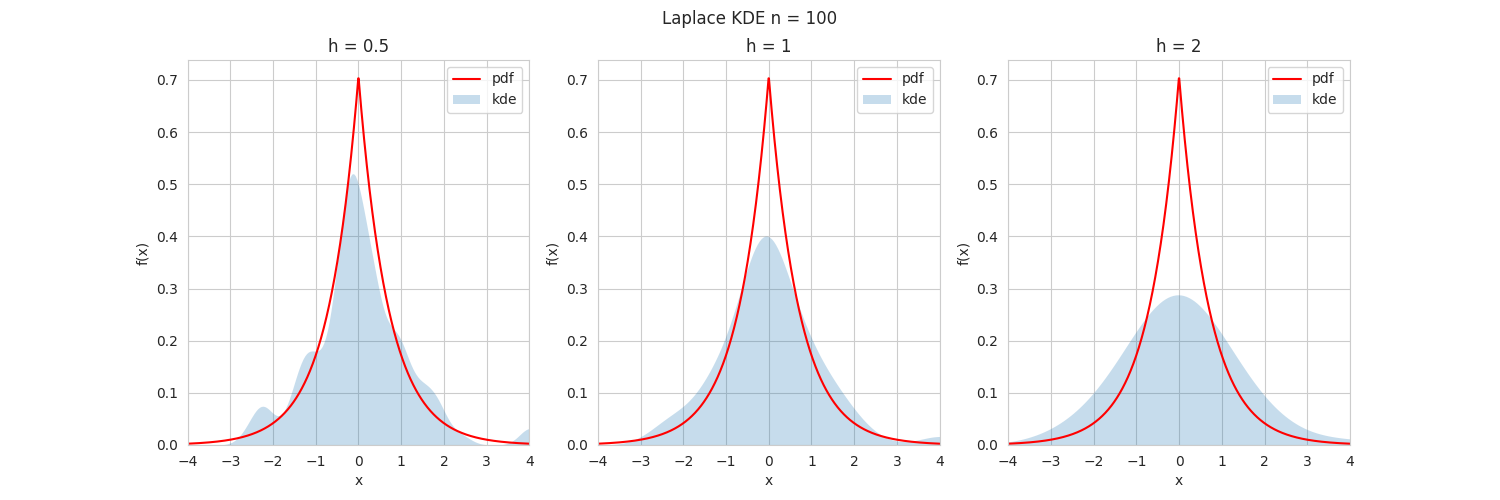
\includegraphics[scale=0.5]{Laplace_pdf_100.png}
    \caption{Распределение Лапласа размерностью 100}
\end{figure}

\begin{figure}[H]
    \centering
    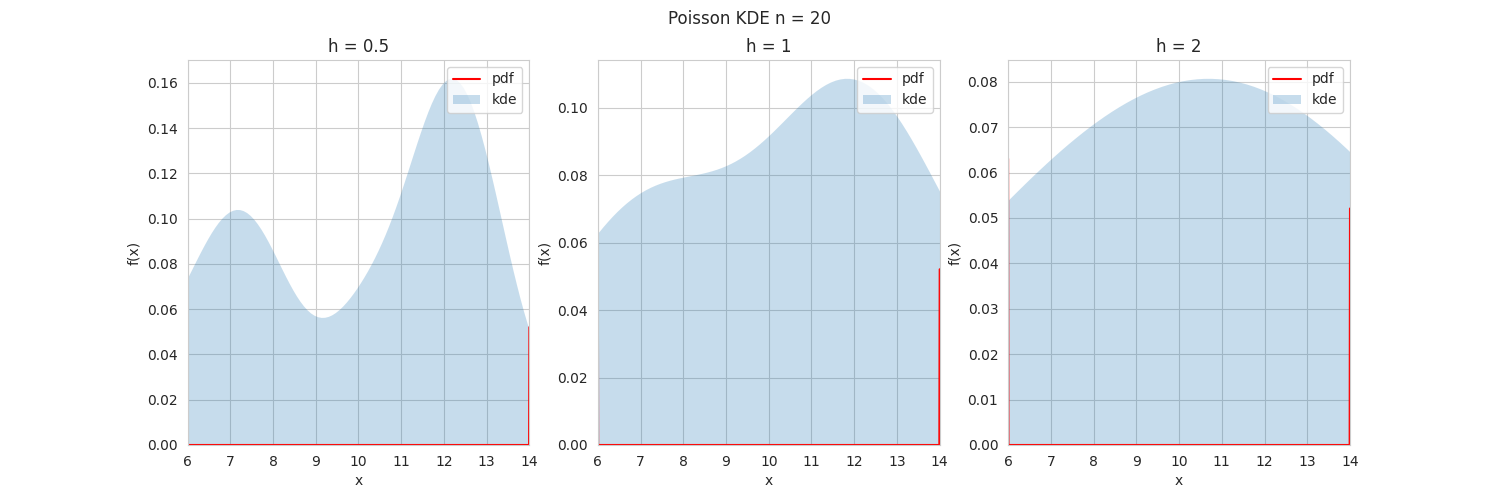
\includegraphics[scale=0.5]{Poisson_pdf_20.png}
    \caption{Распределение Пуассона размерностью 20}
\end{figure}

\begin{figure}[H]
    \centering
    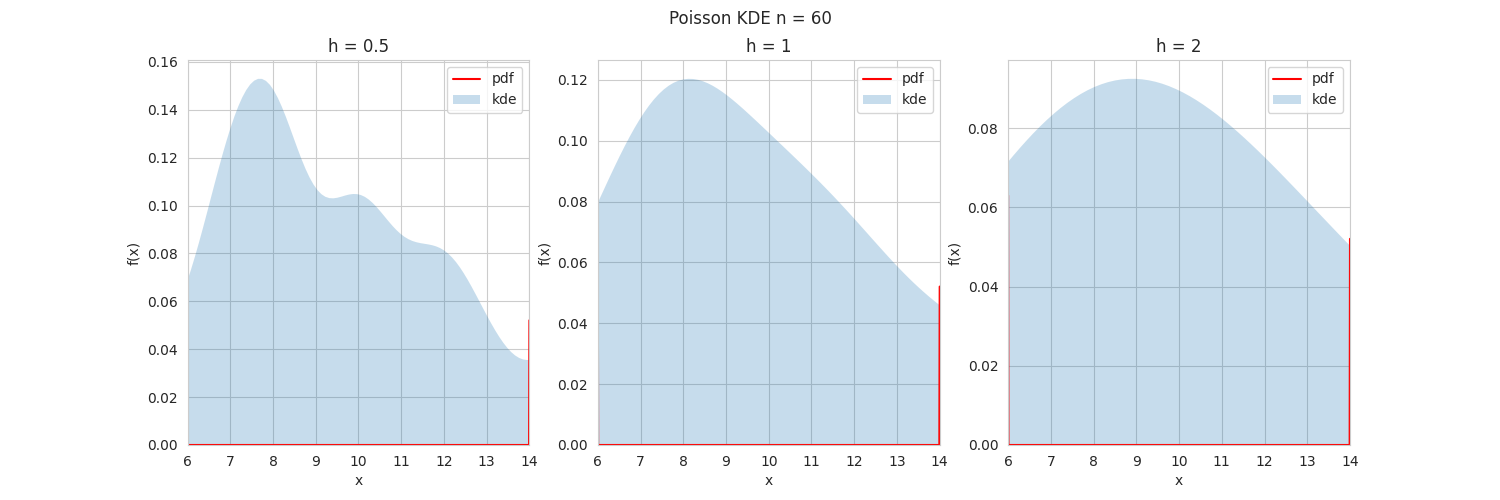
\includegraphics[scale=0.5]{Poisson_pdf_60.png}
    \caption{Распределение Пуассона размерностью 60}
\end{figure}

\begin{figure}[H]
    \centering
    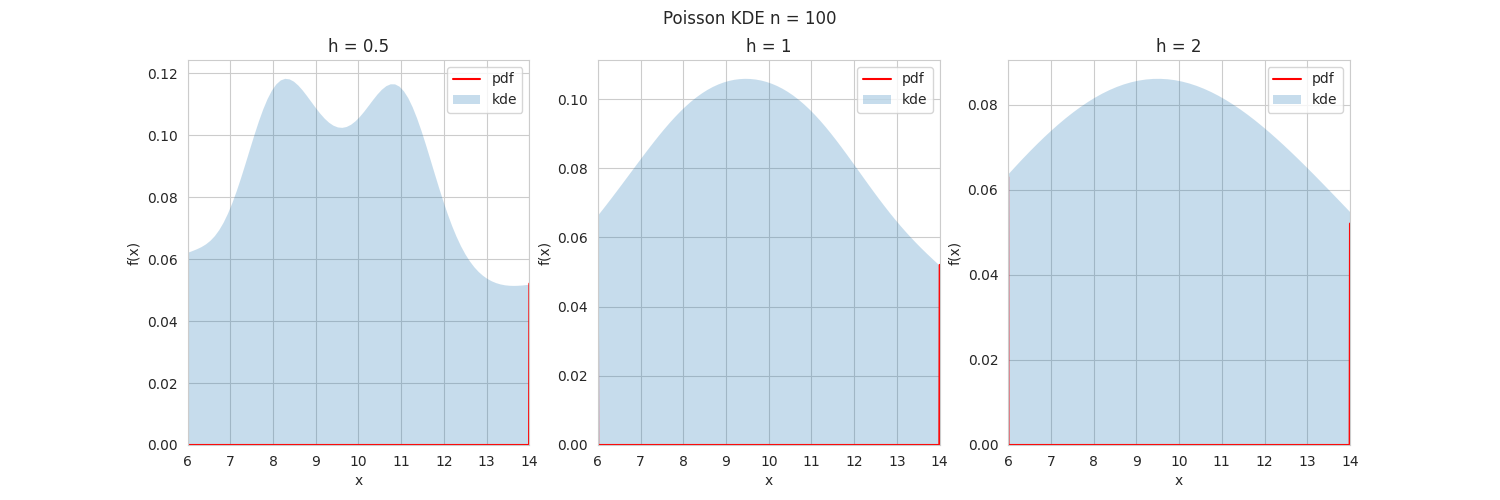
\includegraphics[scale=0.5]{Poisson_pdf_100.png}
    \caption{Распределение Пуассона размерностью 100}
\end{figure}

\begin{figure}[H]
    \centering
    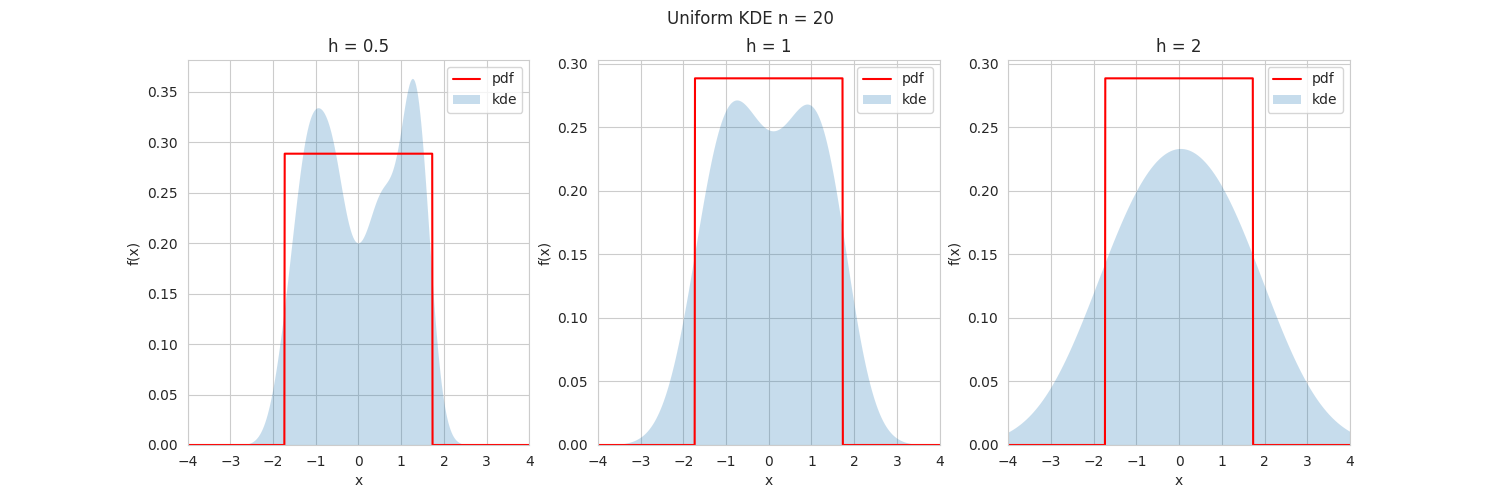
\includegraphics[scale=0.5]{Uniform_pdf_20.png}
    \caption{Равномерное распределение размерностью 20}
\end{figure}

\begin{figure}[H]
    \centering
    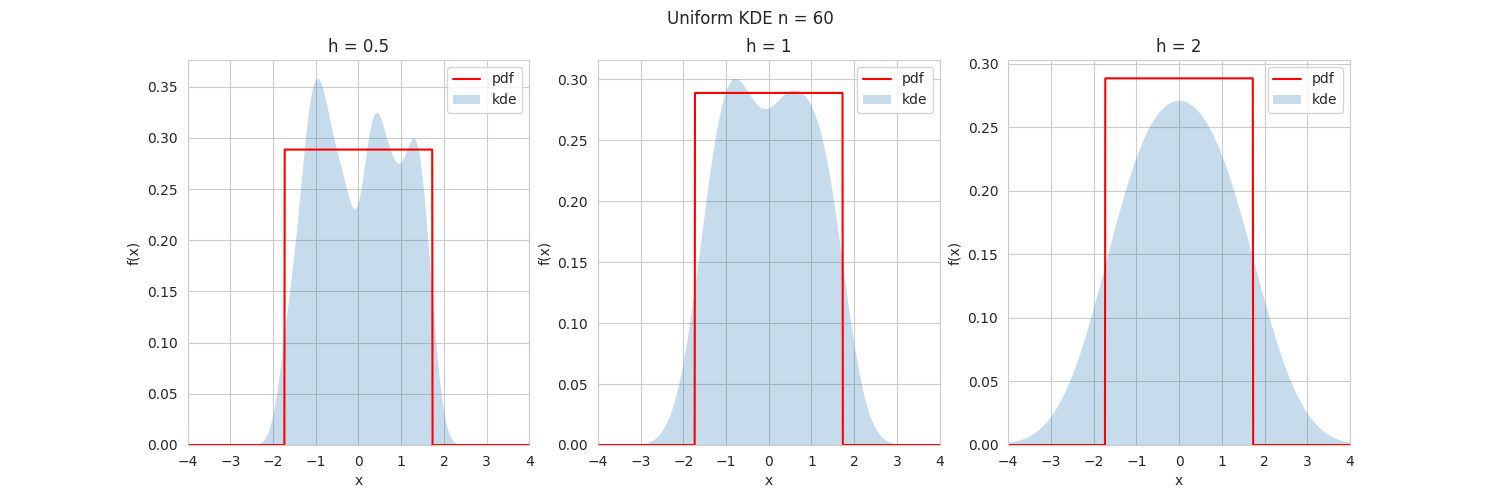
\includegraphics[scale=0.5]{Uniform_pdf_60.png}
    \caption{Равномерное распределение размерностью 60}
\end{figure}

\begin{figure}[H]
    \centering
    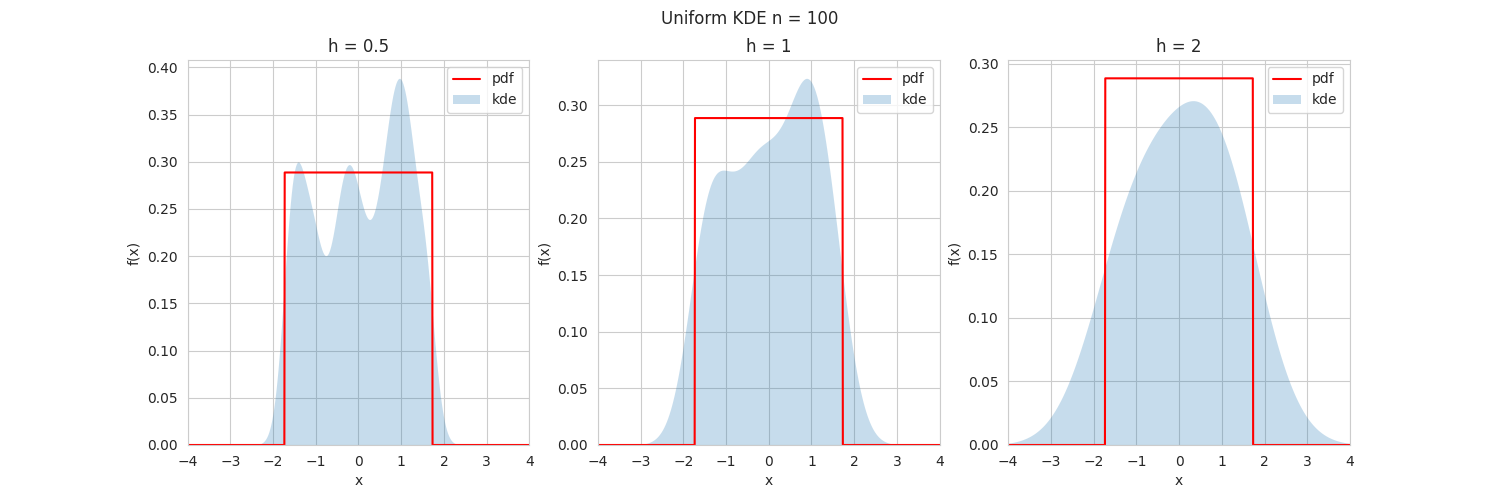
\includegraphics[scale=0.5]{Uniform_pdf_100.png}
    \caption{Равномерное распределение размерностью 100}
\end{figure}

\section{Обсуждение}
На графиках эмпирических функций можно заметить, что с увеличением размерности выборки соответствующая ступенчатая эмпирическая функция становится ближе к эталонной функции распределения. Из представленных распределений график эмпирической функции распределения Пуассона больше всего отклоняется от эталонной функции.

Графики ядерных оценок плотностей распределения тоже показывают приближение ядерной оценки к функции плотности вероятности по всем $h$ при увеличении размерности выборки. При этом для распределения Коши лучшим значением размерности выборки можно считать 60.

Для разных распределений лучшее значение параметра $h$ различается. $h=h_n$ лучше всего приближает нормальное распределение, распределение Пуассона и равномерное распределение. Для распределения Коши и Лапласа оптимально значение $h=\frac{h_n}{2}$. Помимо этого при увеличении параметра $h$ уменьшается значение пиковой точки и расширяется основание графика ядерной оценки для распределения Коши и равномерного. И для всех распределений при значении параметра $h=2h_n$ замечается преобразование графика ядерной оценки в функцию с единственным максимумом.
\end{document}